\documentclass[a4paper,12pt]{article}
\usepackage[utf8]{inputenc}
\usepackage{amsmath}
\usepackage{graphicx}
\usepackage{wrapfig}
\usepackage{geometry}
\usepackage[english]{babel}
\usepackage{physics}
\usepackage{multicol}
\usepackage[square,numbers]{natbib}
%\bibliographystyle{abbrvnat}
 
\geometry{a4paper, margin=1in}

\title{Lennard-Jones Fluids and Monte Carlo Simulation}
\author{
    Julio Fernando Vicente Maldonado \thanks{Escuela de Ciencias Físicas y Matemáticas, Universidad de San Carlos de Guatemala} \\
     Brian David Leiva Berbena\footnotemark[1] \\
    Francisco Toledo\footnotemark[1] \\
    \texttt{joulefvicente@gmail.com, bridleiva@gmail.com, 
      toledo.fran010@gmail.com}
}
\date{\today}

\begin{document}

\maketitle

\begin{abstract}
This report presents a detailed study of Lennard-Jones fluids using Monte Carlo simulations. The aim is to investigate the properties and behavior of these fluids under different conditions. The results are compared with theoretical predictions and previous studies to validate the simulation approach.
\end{abstract}

\section{Introduction}

\begin{multicols}{2}
Lennard-Jones fluids are a type of molecular fluid characterized by the Lennard-Jones potential, which is a mathematical model that approximates the interaction between a pair of neutral atoms or molecules. This potential is given by the equation:
\begin{equation}
    u(r) = 4\epsilon \left[ \left( \frac{\sigma}{r} \right)^{12} - \left( \frac{\sigma}{r} \right)^{6} \right] 
\end{equation}
where \( \epsilon \) is the depth of the potential well, \( \sigma \) is the finite distance at which the inter-particle potential is zero, and \( r \) is the distance between the particles. The \( r^{-12} \) term represents the repulsive forces, while the \( r^{-6} \) term represents the attractive forces \cite{Viot2016}. Due to its simplicity and effectiveness, the Lennard-Jones potential is widely used in molecular simulations to model van der Waals interactions.

In statistical mechanics, we are interested in computing averages of thermodynamic properties as a function of atom positions and momenta. A thermodynamic average that depends only on configurational properties can be computed by evaluating a multivariate integral:
\begin{equation}
    \langle Q \rangle = \int_V Q\qty(\textbf{r}^N)\rho(\textbf{r}^N)d\textbf{r}^N
\end{equation}   
where \( Q\qty(\textbf{r}^N) \) is the thermodynamic quantity of interest that depends only on the configuration, \( \rho\qty( \textbf{r}^N) \) is the probability density, and \( V \) defines the volume of configuration space over which \( \rho \) has support. 

This integral is very challenging to evaluate analytically due to the high dimensionality of the configuration space. However, Monte Carlo integration provides a powerful numerical method to estimate this value. Monte Carlo simulations use random sampling to explore the configuration space and compute these integrals, making them invaluable in studying complex systems where traditional methods fail.

Monte Carlo simulations are a computational technique used to study the thermodynamic properties of Lennard-Jones fluids. These simulations involve generating random configurations of particles and evaluating the energy of each configuration using the Lennard-Jones potential. By accepting or rejecting these configurations based on a probability criterion, we can sample the equilibrium distribution of the system.

In this report, we explore the application of Monte Carlo simulations to Lennard-Jones fluids. We describe the methodology, including the initialization of particle positions, the calculation of the Lennard-Jones potential, and the criteria for accepting new configurations. Our analysis focuses on understanding the behavior of the system at different temperatures and densities, providing insights into the thermodynamic properties and phase behavior of Lennard-Jones fluids \citep{msse2022}.
\end{multicols}
 

 
\section{Methodology}
\subsection{Lennard-Jones Potential}
The Lennard-Jones potential is commonly used in molecular simulations to model nonbonded interactions, including those of noble gases. This potential is given by the equation, again:
\begin{equation}
    u(r) = 4\epsilon \left[ \left( \frac{\sigma}{r} \right)^{12} - \left( \frac{\sigma}{r} \right)^{6} \right]
\end{equation}
where \( \epsilon \) represents the depth of the potential well, \( \sigma \) is the finite distance at which the inter-particle potential is zero, and \( r \) is the distance between particles.

\begin{multicols}{2}
\begin{center}
 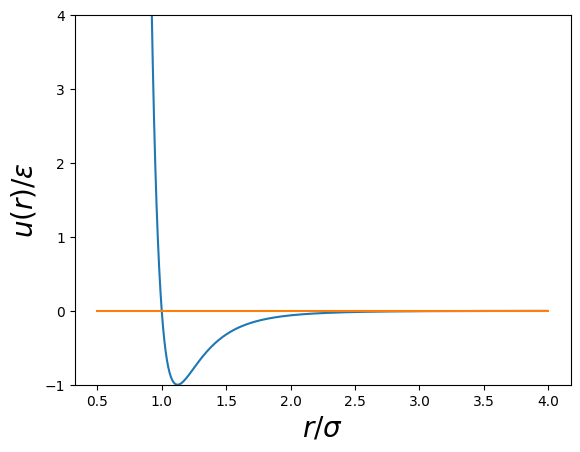
\includegraphics[width = 7.5 cm]{01.png}
\end{center}
The graph shows the reduced Lennard-Jones potential, \( u(r) /\epsilon \), as a function of \( r/\sigma \). All quantities are expressed in dimensionless units: temperature is represented as \( T^* = k_B T/\epsilon \), where \( k_B \) is the Boltzmann constant; distance as \( r^* = r/\sigma \); and energy as \( u^* = u/\epsilon \).

The three-dimensional Lennard-Jones model has a critical point at \( T^* = 1.3 \) and \( \rho^*_c = 0.3 \), and a triple point at \( T^*_t = 0.6 \) and \( \rho^*_t = 0.8 \). For our simulations, we will use the value for the critical point \( T^* = 1.3 \). Consequently, the inverse temperature \( \beta \) is given by:
\begin{equation}
    \beta = \frac{1}{\epsilon k_B T^*}
\end{equation}
Assuming \( \epsilon = k_B = 1 \) in reduced units, then \( \beta = 0.769230 \) \citep{Viot2016}. This value represents the theoretical value for \( \beta \) in our simulation.

For more complex systems, additional energy terms may be included alongside the Lennard-Jones potential. However, for our system of noble gases, the Lennard-Jones potential is the sole contribution to the potential energy.

\end{multicols}



\subsection{Monte Carlo Simulation}
For Lennard-Jones fluids, the Metropolis algorithm is typically used. This involves several key steps.
\begin{multicols}{2}
     The simulation begins with an initial configuration of particles, typically arranged in a cubic box. The Metropolis algorithm then generates new configurations by randomly displacing particles and calculates the resulting energy changes. These changes are accepted or rejected based on the Boltzmann factor, ensuring the system evolves toward equilibrium.

In our simulations, we will use reduced units to simplify the calculations. This involves normalizing quantities by characteristic length ($\sigma$), energy ($\epsilon$), and other relevant parameters of the Lennard-Jones potential\cite{NIST_LJ_Fluid}.

Monte Carlo simulations in the canonical ensemble  for Lennard-Jones fluids involve several detailed steps:
\begin{itemize}
    \item Initialization: Start with a predefined number of particles in a cubic box. Initial positions can be random or based on a lattice structure.
\item Potential Calculation: Compute the pairwise Lennard-Jones potential   $u(r)$, given by equation (1).
\item Metropolis Algorithm: We will expand on this algorithm in the next section 
\item Equilibrium and production: Run the simulation for a sufficient number of steps to reach equilibrium. After equilibrium, collect data to calculate ensemble averages of properties such as energy, average energy and pressure, which are the ones we will consider. 

\end{itemize}

\end{multicols}

\subsection{ The metropolis algorithm}


\subsection{Monte carlo model types}



\section{Results}
The simulation results show the behavior of Lennard-Jones fluids under various temperatures and densities. potential energy, and pressure are calculated and compared with theoretical predictions.


\hspace{1cm}Step 1 \hspace{6cm} step 2


\includegraphics[width=7.5cm]{08.png} 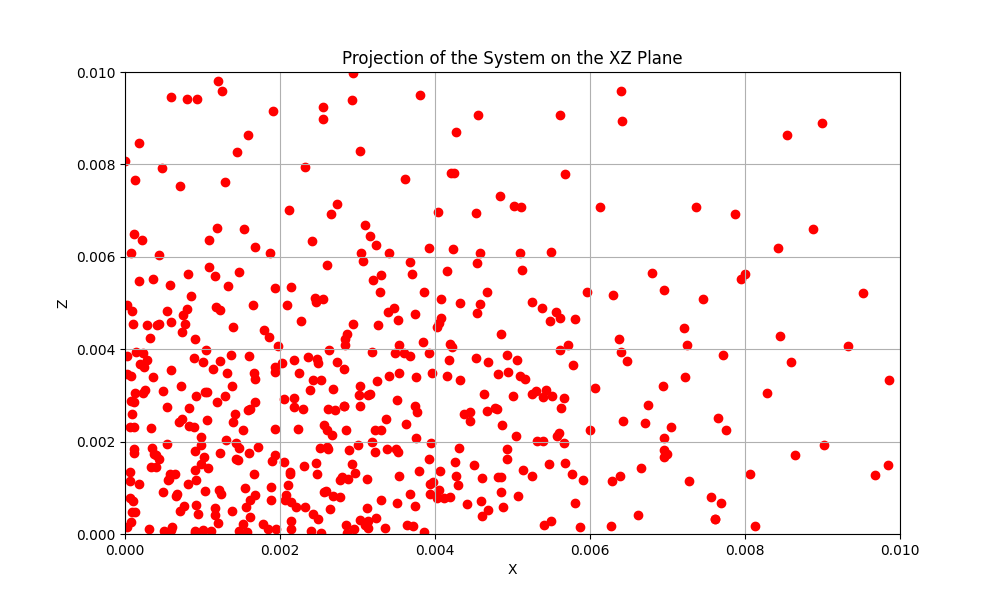
\includegraphics[width=7.5cm]{09.png}
\newpage
Step 3 

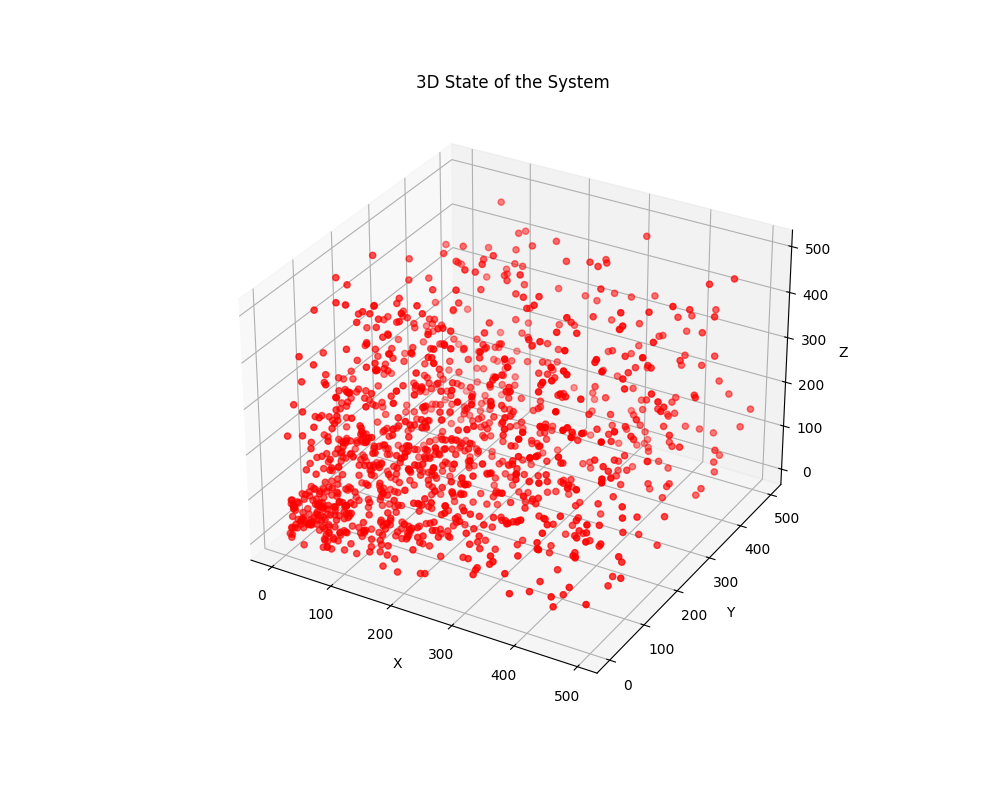
\includegraphics[width=7.5cm]{10.png}
\section{Discussion}
The results demonstrate that Monte Carlo simulations can accurately predict the properties of Lennard-Jones fluids. The agreement with theoretical and previous simulation studies confirms the reliability of the simulation approach. 

\section{Conclusion}
Monte Carlo simulations are an effective tool for studying Lennard-Jones fluids. The findings provide insights into the thermodynamic properties and can be used to model more complex systems. 

\bibliographystyle{plainnat}
\bibliography{referencias}

\end{document}



